\documentclass[border=10pt]{standalone}
\usepackage{tikz}
\usetikzlibrary{arrows.meta,decorations.pathreplacing,calc}
\usepackage{amsmath,amssymb}
\begin{document}
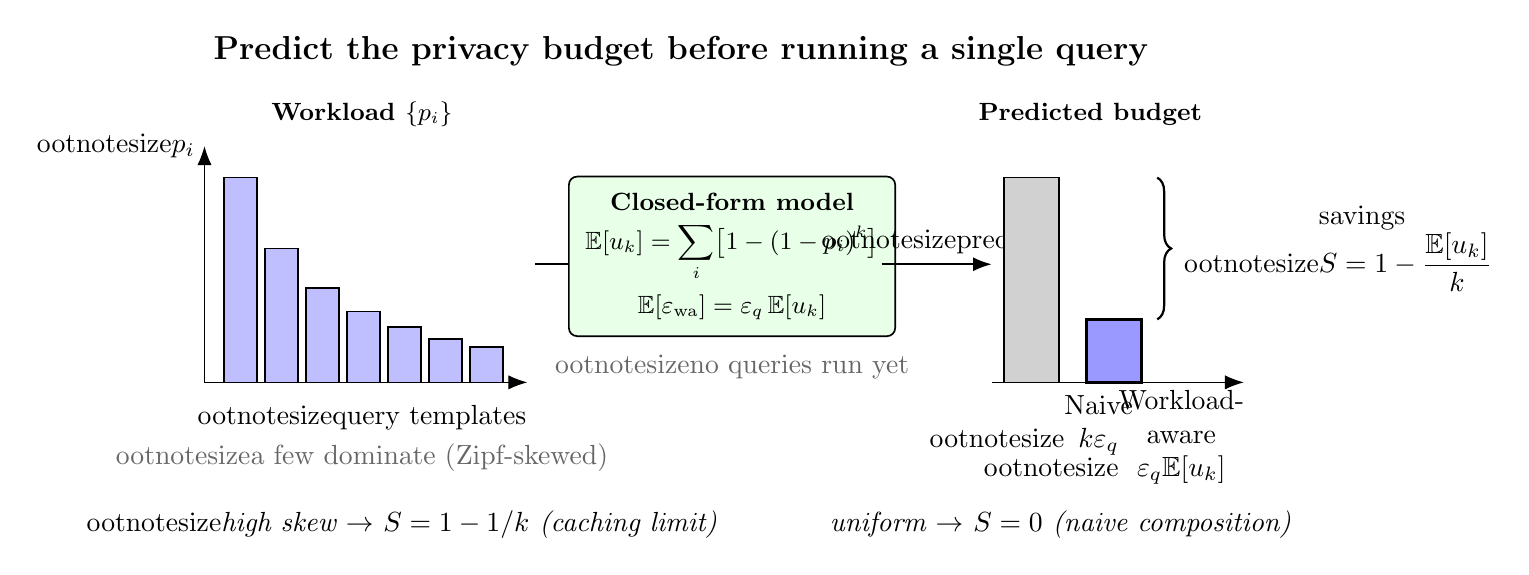
\begin{tikzpicture}[
  font=\small,
  >={Latex[length=2.4mm]},
  modelbox/.style={rectangle, rounded corners=3pt, draw=black, semithick,
                   fill=green!9, align=center, inner sep=6pt},
]
% ===== big title =====
\node[font=\large\bfseries] at (5.9,4.2) {Predict the privacy budget before running a single query};

% ===== Panel 1: workload (Zipf bars) =====
\def\bw{0.42}
\foreach \x/\h in {0.10/2.6, 0.62/1.7, 1.14/1.2, 1.66/0.9, 2.18/0.7, 2.70/0.55, 3.22/0.45}{
  \draw[draw=black, fill=blue!25, semithick] (\x,0) rectangle ++(\bw,\h);
}
\draw[->] (-0.15,0) -- (-0.15,3.0) node[left,font=ootnotesize]{$p_i$};
\draw[->] (-0.15,0) -- (3.95,0);
\node[font=ootnotesize] at (1.85,-0.45) {query templates};
\node[font=ootnotesize, text=black!60] at (1.85,-0.95) {a few dominate (Zipf-skewed)};
\node[font=\small\bfseries] at (1.85,3.4) {Workload $\{p_i\}$};

% arrow to model
\draw[->,thick] (4.05,1.5) -- (4.75,1.5);

% ===== Panel 2: model =====
\node (model) [modelbox] at (6.55,1.6) {%
  \textbf{Closed-form model}\\[3pt]
  $\displaystyle \mathbb{E}[u_k]=\sum_{i}\bigl[1-(1-p_i)^k\bigr]$\\[4pt]
  $\displaystyle \mathbb{E}[\varepsilon_{\mathrm{wa}}]=\varepsilon_q\,\mathbb{E}[u_k]$};
\node[font=ootnotesize, text=black!60] at (6.55,0.2) {no queries run yet};

% arrow to budget bars
\draw[->,thick] (8.45,1.5) -- node[above,font=ootnotesize]{predicts} (9.85,1.5);

% ===== Panel 3: predicted budget bars =====
\def\nh{2.6}
\def\wh{0.8}
\draw[draw=black, fill=black!18, semithick] (10.0,0) rectangle ++(0.7,\nh);
\draw[draw=black, fill=blue!40, very thick] (11.05,0) rectangle ++(0.7,\wh);
\draw[->] (9.85,0) -- (13.05,0);
\node[font=ootnotesize, align=center] at (10.35,-0.55) {Naive\\$k\varepsilon_q$};
\node[font=ootnotesize, align=center] at (11.4,-0.7) {Workload-\\aware\\$\varepsilon_q\mathbb{E}[u_k]$};
\node[font=\small\bfseries] at (11.1,3.4) {Predicted budget};
% savings brace (the gap that the model saves)
\draw[decorate, decoration={brace,amplitude=5pt}, thick] (11.95,\nh) -- (11.95,\wh)
  node[midway, right=6pt, align=left, font=ootnotesize]{savings\\$S=1-\dfrac{\mathbb{E}[u_k]}{k}$};

% ===== bottom spectrum strip =====
\node[font=ootnotesize\itshape, align=center] at (6.0,-1.8)
  {high skew $\rightarrow$ $S=1-1/k$ (caching limit)\qquad\qquad uniform $\rightarrow$ $S=0$ (naive composition)};
\end{tikzpicture}
\end{document}
